\documentclass[twoside]{article}

\usepackage{aistats2023}
% If your paper is accepted, change the options for the package
% aistats2023 as follows:
%
%\usepackage[accepted]{aistats2023}
%
% This option will print headings for the title of your paper and
% headings for the authors names, plus a copyright note at the end of
% the first column of the first page.

% If you set papersize explicitly, activate the following three lines:
%\special{papersize = 8.5in, 11in}
%\setlength{\pdfpageheight}{11in}
%\setlength{\pdfpagewidth}{8.5in}

% If you use natbib package, activate the following three lines:
\usepackage[round]{natbib}
\renewcommand{\bibname}{References}
\renewcommand{\bibsection}{\subsubsection*{\bibname}}
\bibliographystyle{plainnat}
\usepackage{amsmath}
\usepackage{amssymb}
\usepackage{xfrac}
\usepackage{hyperref}
\usepackage{graphicx}
\graphicspath{ {./../examples/} }
% If you use BibTeX in apalike style, activate the following line:
%\bibliographystyle{apalike}

\usepackage{tikz}
\usetikzlibrary{matrix,positioning,arrows.meta,arrows,fit,backgrounds,decorations.pathreplacing}
\tikzset{ mymat/.style={ matrix of math nodes, text height=2.5ex, text
depth=0.75ex, text width=6.00ex, align=center, column
sep=-\pgflinewidth, nodes={minimum height=5.0ex} }, mymats/.style={
mymat, nodes={draw,fill=#1} }, mymat2/.style={ matrix of math nodes,
text height=1.0ex, text depth=0.0ex, minimum width=5ex, % text
width=7.00ex, align=center, column sep=-\pgflinewidth }, }
\usetikzlibrary{shapes.geometric, arrows, backgrounds, scopes}
\usepackage{pgfplots} \pgfplotsset{width=6.75cm, compat=newest}
\usepackage[utf8]{inputenc} \DeclareUnicodeCharacter{2212}{−}
\usepgfplotslibrary{groupplots,dateplot}
\usetikzlibrary{patterns,shapes.arrows}



\newcommand{\dfdx}{f^s}
\newcommand{\xc}{\mathbf{x}_c}
\newcommand{\DY}{\mathbf{\Delta Y}}
\newcommand{\xb}{\mathbf{x}}
\newcommand{\Xcb}{\mathbf{X}_c}
\newcommand{\Xb}{\mathcal{X}}

\begin{document}

% If your paper is accepted and the title of your paper is very long,
% the style will print as headings an error message. Use the following
% command to supply a shorter title of your paper so that it can be
% used as headings.
%
%\runningtitle{I use this title instead because the last one was very long}

% If your paper is accepted and the number of authors is large, the
% style will print as headings an error message. Use the following
% command to supply a shorter version of the authors names so that
% they can be used as headings (for example, use only the surnames)
%
%\runningauthor{Surname 1, Surname 2, Surname 3, ...., Surname n}

\twocolumn[

\aistatstitle{Uncertainty-aware Accumulated Local Effects (UALE) for quantifying the hetegeneity of instance-level feature effects}

\aistatsauthor{ Author 1 \And Author 2 \And  Author 3 }

\aistatsaddress{ Institution 1 \And  Institution 2 \And Institution 3 } ]

\begin{abstract}

Accumulated Local Effects (ALE) is a popular approach to explainable AI that quantifies how a feature influences the decisions of a model taking into account feature correlations. However, in case of strong interactions between features, instance-level feature effects may deviate from the average curve provided by ALE. Therefore, it is crucial to quantify this deviation, namely, the uncertainty of the effect. In this work, we define Uncertainty-aware ALE (UALE) to quantify and visualize, on a single plot, both the average effect and the uncertainty. Furthermore, as in ALE, UALE's approximation requires partitioning the feature domain into non-overlapping intervals (bin-splitting). The average effect and the uncertainty are then computed from the instances that lie in each bin.  In this work, we formally prove that to achieve an unbiased approximation of the uncertainty in each bin, bin-splitting must follow specific constraints. Based on this, we propose a method for automatically finding the optimal intervals, balancing the trade-off between estimation bias and variance. We demonstrate through synthetic and real datasets (a) the advantages of modelling the uncertainty with UALE compared to other methods and (b) the importance of appropriate bin splitting for an accurate approximation of the mean effect and uncertainty.
\end{abstract}


\section{INTRODUCTION}

Recently, Machine Learning (ML) has been adopted in critical domains,
such as healthcare and finance. In these areas, we need a combination
of accurate predictions along with meaningful explanations to support
them. For this reason there is an increased interest in Explainable AI
(XAI), to understand the decision mechanism of 
%the field that provides interpretations about the behavior of
complex black-box models. XAI literature distinguishes between local
and global explainability
techniques~\citep{Molnar2020interpretable}. Local methods explain the prediction of a
specific instance, whereas global methods provide an explanation that summarizes the entire model behavior. Global methods provide a universal explanation, aggregating the various local explanations into a single interpretable outcome,
usually a number or a plot. If users want to get a rough overview
about which features are significant (feature importance) or whether a
particular feature has a positive or negative effect on the output
(feature effect), they should opt for a global explainability
technique. On the other hand, aggregating the individual explanations
is vulnerable to misinterpretations. Under strong interactions and
correlations between features, the global explanation may obfuscate
heterogeneous effects that exist under the
hood~\citep{herbinger2022repid}; a phenomenon called \emph{aggregation
bias}~\citep{mehrabi2021survey}.

Feature effect (FE) \citep{Gromping2020MAEP} is a fundamental category of global
explainability methods aiming at isolating the impact
of a single feature on the output\footnote{Often, FE methods also
  isolate the combined effect of a pair of features to the
  output. Combinations of more than two features are uncommon, since they are difficult to estimate and visualize.}.
FE methods suffer from aggregation bias because, often, implications of the average effect on the model behavior are unclear. For example, a feature with zero average effect may indicate no effect on the output or, 
a highly positive effect in some cases and a highly negative effect in others. 
There are
three widely-used FE methods: \emph{Partial Dependence Plots}
(PDP)\citep{friedman2001greedy}, \emph{Marignal Plots}
(MP)\citep{apley2020visualizing} and \emph{Aggregated Local Effects}
(ALE)\citep{apley2020visualizing}. PDP and MP have been criticized \todo{Add a reference}for
computing erroneous effects when the input features are (highly)
correlated, which is typical in many ML cases. Therefore,
ALE has been established as the state-of-the-art FE method. However, ALE faces two crucial limitations, the first concerns ALE
definition and the second one ALE approximation. Regarding the
definition, ALE does not inform the user about the uncertainty, i.e.,
the level of heterogeneous effects hidden behind the average effect
due to implicit feature interactions. In contrast, in PDPs the
heterogeneous effects can be identified by exploring the
Individual Conditional Expectations
(ICE)~\citep{goldstein2015peeking}. Regarding the approximation,
i.e.~the estimation using the (limited) samples of the training set,
ALE requires an additional \textit{bin-splitting} step to partition the domain of the feature of interest into consecutive non-overlapping intervals (regions) and to estimate a
constant effect in each region. The effect is estimated from the population of samples that fall
inside the region. Specifying an appropriate set of bins is of particular
importance, since ALE's interpretation is meaningful only inside each
region~\citep{molnar2022}. However, this crucial step has not raised
the appropriate attention and the approximation is vulnerable to
potential misinterpretations.\todo{I miss what exactly is the simplication of existing mehtods here. Should we add e.g., typically equisized bins?}

In this paper, we present Uncertainty-aware Accumulated Local Effects
(UALE) an extension of ALE for measuring the uncertainty of the
explanation, i.e.~how certain we are that the average explanation
would predict the feature effect to an instance drawn at random. We
show that choosing an appropriate sequence of intervals is
particularly important for a robust and unbiased estimation of the
uncertainty and we provide an algorithm that automates this step. We
also formally prove the bin-splitting conditions for an unbiased
estimation of the uncertainty. We apply our method in multiple
synthetic and real world datasets for evaluating its performance.

\paragraph{Contributions.} The contributions of this paper are:

\begin{itemize}
\item UALE, a FE method that extends ALE for quantifying the
  heterogeneous effects (uncertainty).
\item A formal proof of the bin-splitting requirements for an unbiased
  approximation of the heterogeneous effects.
\item A framework for automatically extracting regions with similar
  effects, improving the estimation and the interpretability of ALE
  plots.
\end{itemize}

We provide empirical evaluation of the method in artificial and real
datasets. The implementation of our method and the code for
reproducing all the experiments is provided in the submission and will
become publicly available upon acceptance.


\section{BACKGROUND AND RELATED WORK}

In this section, we describe the basic methods for FE and uncertainty
quantification, focusing on ALE definition. We, then, review the ALE
approximation\citep{apley2020visualizing, gkolemis22}, describing some
of its vulnerabilities.

\paragraph{Notation.} We refer to random variables (rv) using
uppercase \( X \), to simple variables with plain lowercase \( x \)
and to vectors with bold \( \xb \). Often, we partition the input
vector \(\xb \in \mathbb{R}^D\) to the feature of interest
\(x_s \in \mathbb{R} \) and the rest of the features
\(\xc \in \mathbb{R}^{D-1}\). For convenience we denote it as
\((x_s, \mathbf{x}_c)\), but we clarify that it implies the vector
\((x_1, \cdots , x_s, \cdots, x_D)\). Equivalently, we denote the
corresponding rv as \(\mathbf{X} = (X_s, \mathbf{X}_c)\). When we
refer to an instance of the training set, we use
\(\xb^i= (\xc^i, x_s^i) \). The black-box function is
\(f : \mathbb{R}^D \rightarrow \mathbb{R}\) and the FE of the \(s\)-th
feature is \(f^{\mathtt{<method>}}(x_s)\), with \(\mathtt{<method>}\)
indicating the particular method in use.\footnote{An extensive list of all
  symbols used in the paper is provided at the Appendix.}

\subsection{Feature Effect Methods And ALE Definition}
\label{sec:feat-effect-meth}

The three well-known feature effect methods are: PDP, MP and ALE. PDP
formulates the FE of the \(s\)-th attribute as an expectation over the
marginal distribution \(\mathbf{X}_c\), i.e.,
\(f^{\mathtt{PDP}}(x_s) =
\mathbb{E}_{\mathbf{X}_c}[f(x_s,\mathbf{X}_c)]\), whereas MP
formulates it as an expectation over the conditional
\(\mathbf{X}_c|X_s\), i.e.,
\(f^{\mathtt{MP}}(x_s) = \mathbb{E}_{\mathbf{X}_c|x_s}[f(x_s,
\mathbf{X}_c)]\). ALE defines the local effect of the \(s\)-th feature
at point \(x_s = z\) as
\(f^s(z, \xc) = \frac{\partial f}{\partial x_s} (z, \xc)\). All the
local explanations at \(z\) are, then, weighted by the conditional
distribution \(p(\xc|x_s=z)\) and are averaged, to produce the
averaged effect \(\mu(z)\). ALE is the accumulation of the averaged
local effects:

\begin{equation}
  \label{eq:ALE}
  f^{\mathtt{ALE}}(x_s) = \int_{x_{s,min}}^{x_s} \underbrace{\mathbb{E}_{\Xcb|X_s=z}\left [f^s (z, \Xcb)\right ]}_{\mu(z)} \partial z
\end{equation}


Eq.~(\ref{eq:ALE}) has specific advantages which gain particular value in cases of
correlated input features. In these cases, PDP integrates over
unrealistic instances due to the use of the marginal distribution
\(\mathbf{X}_c \), and MP computes aggregated effects, i.e., imputes
the combined effect of sets of features to a single feature. ALE
manages to resolve both issues, and is therefore the most trustable
method in cases of correlated features.

\subsection{Quantification Of Heterogeneous Effects.}
\label{sec:quant-heter-effects}

FE methods reply to the question \textit{what is the average (global)
  effect on the output, if the value of a specific feature is
  increased/decreased}. It comes naturally to also ask \textit{to what
  extent the local effects deviate from the global
  explanation}. Quantifying the uncertainty of the global explanation
has attracted a lot of interest. ICE and
d-ICE\citep{goldstein2015peeking} provide a set of curves that are
plot on top-of the PDP. Both methods produce one curve for each
instance of the training set;
\(f^{\mathtt{ICE}}_i(x_s) = f(x_s, \xc^i)\) for ICE and
\(f^{\mathtt{d-ICE}}_i(x_s) = \frac{\partial f}{\partial x_s} (x_s,
\xc^i)\) for d-ICE. The user then visually observes if the curves are
homogeneous and to what extent they deviate from the PDP. Some methods
try to automate the aforementioned visual exploration, by grouping
(d-)ICE plots into clusters~\citep{molnar2020model,
  herbinger2022repid, britton2019vine}. Some other approaches, like
H-Statistic\citep{friedman2008predictive}, Greenwell's interaction
index\citep{greenwell2018simple} or SHAP interaction
values\citep{lundberg2018consistent}, quantify the level of
interaction between the input features, with an interaction value. A
strong interaction index is an indicator for the existence of
heterogeneous effects.

The aforementioned approaches are under two limitations; They either
do not quantify the uncertainty of the FE directly or they are based
on PDPs, and, therefore, they are subject to the failure modes of PDPs
in cases of correlated features\citep{baniecki2021fooling}, as we will
show in-depth in Section~\ref{sec:simulation-examples-1}. To the best
of our knowledge, no work exist so far that quantifies the
heterogeneous effects based on the formulation of ALE.

\subsection{ALE Approximation.}
\label{sec:ale-approximation}

In ML scenarios, ALE is estimated from the training set
examples. Therefore, \citep{apley2020visualizing} proposed dividing
the feature domain in \(K\) equal-sized bins and estimating the local effects in
each bin by evaluating the black box-function at the bin limits:
\begin{equation}
  \label{eq:ALE_accumulated_mean_est}
  \hat{f}^{\mathtt{ALE}}(x_s) = \sum_{k=1}^{k_x} \frac{1}{|\mathcal{S}_k|} \sum_{i:\mathbf{x}^i \in
    \mathcal{S}_k} \left [ f(z_{k}, \xc^i) - f(z_{k-1}, \xc^i)) \right ]
\end{equation}
We denote as \(k_x\) the index of the bin that \(x_s\) belongs to,
i.e. \(k_x: z_{k_x-1} \leq x_s < z_{k_x} \) and \(\mathcal{S}_k\) is
the set of training instance that lie in the \(k\)-th bin, i.e.
\( \mathcal{S}_k = \{ \xb^i : z_{k-1} \leq x^i_s < z_{k} \}
\). Afterwards,~\citep{gkolemis22} proposed the Differential ALE
(DALE) that computes the local effects on the training instances using
auto-differentiation:
\begin{equation}
  \label{eq:DALE_accumulated_mean_est}
  \hat{f}^{\mathtt{DALE}}(x_s) = \Delta x \sum_{k=1}^{k_x} \frac{1}{|\mathcal{S}_k|} \sum_{i:\mathbf{x}^i \in
    \mathcal{S}_k} f^s(\mathbf{x}^i)
\end{equation}
%
Their method has the advantages of remaining on-distribution even when
bins become wider and, most importantly, allows the recomputation of
the accumulated effect with different bin-splitting with near-zero
computational cost.

Both approximations ask from the user to blindly decide the number of
bins, denoted with \(K\), for splitting the axis into equally-sized
bins. This approach introduces significant limitations. Specifically, setting \(K\) to a small
value may hide fine-grain effects due to large bins while setting \(K\)
to a high value leads to poor bin-effect estimations from limited
samples. In general, the user may face contradictory explanations for
different \(K\) without a clue for which one to trust.

\section{Uncertainty-Aware ALE (UALE)}
\label{sec:UALE}

UALE extends ALE for quantifying the level of heterogeneous effects
(uncertainty) and automates the bin-splitting. At
Section~\ref{sec:UALE-definition-1} we define UALE, at
Section~\ref{sec:UALE-definition-2} we redefine it using an
interval-based formulation, at
Section~\ref{sec:UALE-approximation} we provide an
approximation and at Section~\ref{sec:bin-spliting} we define and
solve the problem of optimal bin-splitting.

\subsection{UALE: ALE With Uncertainty Quantification}
\label{sec:UALE-definition-1}

We extend ALE definition of Eq.~(\ref{eq:ALE}) with a component for
quantifying the uncertainty. We denote as \(\mathcal{H}(z)\) the
uncertainty of the local effects at a specific point \(x_s=z\) and we
quantify it as the standard deviation of the local explanations
\(\mathcal{H}(z) = \sigma(z)\), where:

\begin{equation}
  \label{eq:ALE_var}
  \sigma^2(z) = \mathbb{E}_{\Xcb|z}\left [ \left (\dfdx (z, X_c) - \mu(z) \right )^2 \right ] 
\end{equation}
\noindent
The uncertainty emerges from the natural characteristics of the
experiment, i.e.,~the feature correlations existent in the data
generating distribution and the implicit interactions of the black-box
function. We also define the accumulated uncertainty at \(x_s\), as
the accumulation of the standard deviation of the local effects along
the axis:
\begin{equation}
  \label{eq:ALE_acc_unc}
  f^{\mathtt{ALE}}_{\sigma}(x_s) = \int_{x_{s, min}}^{x_s} \sigma(z) \partial z
\end{equation}
\noindent
UALE formulates the effect at a specific point \(x_s\) with a compact
tuple that consists of the average effect and the uncertainty
\((\mu(z), \sigma(z))\) and visualizes them as a continuous curve with
a confidence region, i.e.
\(f^{\mathtt{UALE}}(x_s) := f^{\mathtt{ALE}}_{\mu}(x_s) \pm
f^{\mathtt{ALE}}_{\sigma}(x_s)\).

\subsection{Interval-Based Formulation and Approximation}
\label{sec:UALE-definition-2}

In real scenarios, all estimations are based on the instances of the
training set. Therefore, we cannot estimate \(\mu(z), \sigma(z)\) at
the granularity of a point, because the probability of observing a
sample inside the region \([x_s - h, x_s + h]\) tends to zero, when
\(h \to 0\). We define the regional-effect \(\mu(z_1, z_2)\) and the
regional-uncertainty \(\mathcal{H}(z_1, z_2) = \sigma(z_1, z_2)\), as the summary statistics
that characterize the effect and the uncertainty inside the interval
\([z_1, z_2)\):

\begin{equation}
  \label{eq:mu_bin}
    \mu(z_1, z_2) = \mathbb{E}_{z \sim \mathcal{U}(z_1,z_2)} [\mu(z)]
    = \frac{\int_{z_1}^{z_2} \mu(z) \partial z}{z_2 - z_1}
\end{equation}

\begin{equation}
  \label{eq:var_bin}
  \sigma^2(z_1, z_2) = \mathbb{E}_{z \sim \mathcal{U}(z_1,z_2)} [\sigma^2(z)] =  \frac{\int_{z_1}^{z_2} \sigma^2(z)  \partial z}{z_2 - z_1}
\end{equation}

%
Intuitively, the regional-effect and the regional-uncertainty quantify
the expected average effect and the expected uncertainty if we
randomly draw a point \(z^*\) given a uniform distribution
\(z^* \sim \mathcal{U}(z_1, z_2)\). If we also define as
\(\mathcal{Z}\) the sequence of \(K+1\) points that partition the
domain of the \(s\)-th feature into \(K\) variable-size intervals,
i.e.  \(\mathcal{Z} = \{z_0, \ldots, z_K\}\), we can redefine UALE
using an interval-based formulation
\(\tilde{f}^{\mathtt{UALE}}_{\mathcal{Z}}(x_s):= \tilde{f}^{\mathtt{ALE}}_{\mathcal{Z}, \mu}(x_s)
\pm \tilde{f}^{\mathtt{ALE}}_{\mathcal{Z}, \sigma}(x_s)\), where:

\begin{equation}
  \label{eq:ALE_2}
  \tilde{f}^{\mathtt{ALE}}_{\mathcal{Z}, \mu}(x_s) = \sum_{k=1}^{k_x} \mu(z_{k-1}, z_k) (z_k - z_{k-1})
\end{equation}

\begin{equation}
  \label{eq:ALE_accumulated_var}
  \tilde{f}^{\mathtt{ALE}}_{\mathcal{Z}, \sigma}(x_s) =  \sum_{k=1}^{k_x} \sigma(z_{k-1}, z_k) (z_k - z_{k-1})
\end{equation}
%

\subsection{Interval-Based Approximation}
\label{sec:UALE-approximation}

For approximating the mean effect (Eq.~\eqref{eq:mu_bin}) and the
uncertainty (Eq.~\eqref{eq:var_bin}) we use the set \(\mathcal{S}_k\)
of dataset instances with the \(s\)-th feature lying inside the
interval
\( \mathcal{S}_k= \{ \mathbf{x}^i : z_{k-1} \leq x^i_s < z_k \} \):

\begin{equation}
  \label{eq:2}
  \hat{\mu}(z_{k-1}, z_k) = \frac{1}{|\mathcal{S}_k|}
  \sum_{i:\mathbf{x}^i \in \mathcal{S}_k} \left [ \dfdx(\mathbf{x}^i)
  \right ]
\end{equation}
%
\begin{equation}
  \label{eq:3}
  \hat{\sigma}^2(z_{k-1}, z_k) = \frac{1}{|\mathcal{S}_k|}
\sum_{i:\mathbf{x}^i \in \mathcal{S}_k} \left ( \dfdx(\mathbf{x}^i) -
  \hat{\mu}(z_1, z_2) \right )^2
\end{equation}

Eq.\eqref{eq:2} is an unbiased estimator of Eq.~(\ref{eq:mu_bin})
under the assumption that the points are uniformly distributed inside
the intervals. The same does not hold in the general case for
Eq.\eqref{eq:3}. In the general case, \(\hat{\sigma}^2(z_{k-1}, z_k)\)
is an unbiased estimator of the \textit{observable} variance
\(\sigma^2_{obs}(z_1, z_2) = \frac{\int_{z_1}^{z_2}
    \mathbb{E}_{\xc|x_s=z} \left [ (f^s(z, \xc) - \mu(z_1, z_2) )^2
    \right] \partial z}{z_2 - z_1}\), which as we prove in Theorem 1
is an overestimation of \(\sigma^2(z_1, z_2)\).

\paragraph{Theorem 1.}
\label{sec:theorem-1}

\textit{If we define the residual \(\rho(z)\) as the difference
  between the expected effect at \(x_s\) and the regional effect, i.e
  \(\rho(z) = \mu(z) - \mu(z_1, z_2)\), then the regional variance
  \(\sigma^2(z_1, z_2)\) equals to:}

\begin{equation}
    \label{eq:bin-uncertainty-proof}
 \sigma_{obs}^2(z_1, z_2) = \sigma^2(z_1, z_2) + \frac{\int_{z_1}^{z_2}\rho^2(z) \partial z}{z_2 - z_1}
\end{equation}
\noindent
Theorem 1 reveals an important connection between the ground-truth and
the observable uncertainty inside a region. For convenience, we denote
as
\(\mathcal{E}^2(z_1, z_2) = \frac{\int_{z_1}^{z_2}\rho^2(z) \partial
  z}{z_2 - z_1}\) the error term that models the expected square
residual inside the interval and as
\(\mathcal{H}_{obs}(z_1, z_2) := \sigma_{obs}(z_1, z_2)\) the
observable uncertainty. It holds that the observable uncertainty is an
overestimation of the correct uncertainty

\begin{equation}
  \label{eq:uncertainty-bin}
  \mathcal{H}^2_{obs}(z_1, z_2) = \mathcal{H}^2(z_1, z_2) + \mathcal{E}^2(z_1, z_2)
\end{equation}
%
and, therefore, the estimation is unbiased only in case
\(\mathcal{E}^2(z_1, z_2) = 0\).

\subsection{Bin-Splitting: Finding Regions With Homogeneous Effects}
\label{sec:bin-spliting}

In this section we formulate bin-splitting as an unsupervised
clustering problem, searching for a solution that compromises two
contradictory objectives. On the one hand, we want to minimize the
error term \(\mathcal{E}\) for approaching an unbiased estimation and
on the other hand, we want wide-enough bins for including a fair
population of samples for a robust estimation of
\(\hat{\mu}(z_1, z_2), \hat{\sigma}(z_1, z_2)\). We set-up the
following optimization problem:

\begin{equation}
  \label{eq:opt}
\begin{aligned}
  \min_{ \mathcal{Z} = \{z_0, \ldots, z_K\}} \quad & \mathcal{L} = \sum_{k=1}^K \tau_k \hat{\sigma}^2(z_{k-1}, z_k) \Delta z_k \\
  \textrm{where} \quad & \Delta z_k = z_k - z_{k-1} \\
  & \tau_k = 1 - \alpha \frac{|S_k|}{N} \\
  \textrm{s.t.} \quad & |\mathcal{S}_k| \geq N_{\mathtt{NPB}}\\
                                     & z_0 = x_{s,min}\\
                                     & z_K = x_{s, max}
\end{aligned}
\end{equation}
%
We search for the sequence of intervals \(z_0, \ldots, z_K\) that
minimizes the sum of the bin costs. The cost of each bin is the
approximated variance \(\hat{\sigma}^2_k\) scaled by the bin length
\(\Delta z_k\) and discounted by the term \(\tau_k\). The term
\(\tau_K\) favors the selection of a bigger bin in case it has similar
variance with the aggregate variance of many smaller ones. The
constraint of at least \(N_{\mathtt{PPB}}\) points per bin sets the
lowest-limit for a \textit{robust} estimation. The user can choose to
what extent they favor the creation of wide bins through the discount
parameter by setting the parameter \(\alpha\) and where they set the
minimum for robust approximation with the parameter
\(N_{\mathtt{PPB}}\). For providing a rough idea, in our experiments
we set \(\alpha = 0.2\) which means that the discount ranges between
\([0\%, 20\%]\) and \(N_{\mathtt{PPB}} = \frac{N}{20}\). It is also
important to clarify that by minimizing
\(\hat{\sigma}^2_k \approx \mathcal{H}_{obs}^2\), we actually minimize
the squared error term \(\mathcal{E}^2\), since the term
\(\mathcal{H}^2_{true}\) is independent of the bin splitting.

\subsubsection{Solve Bin-Splitting with Dynamic Programming}
\label{sec:dynamic-programing}

For achieving a computationally-grounded solution we set a threshold
\(K_{max}\) on the maximum number of bins which also discretizes the
solution space. The width of the bin can take discrete values that are
multiple of the minimum step
\(u = \frac{x_{s, max} - x_{s, min}}{K_{max}}\). For defining the
solution, we use two indexes. The index
\(i \in \{0, \ldots, K_{max}\}\) denotes the point \((z_i)\) and the
index \(j \in \{0, \ldots, K_{max}\} \) denotes the position of the
\(j\)-th multiple of the minimum step, i.e., 
\(x_j = x_{s,min} + j \cdot u\). The recursive cost function
\(T(i,j)\) is the cost of setting \(z_i=x_j\):
\begin{equation}
  \label{eq:recursive_cost}
  \mathcal{T}(i,j) = \mathrm{min}_{l \in \{0, \ldots, K_{max}\}} \left [ \mathcal{T}(i-1, l) + \mathcal{B}(x_l, x_j) \right ]
\end{equation}
%
where \(\mathcal{T}(0,j)\) equals zero if \(j=0\) and \(\infty\) in
any other case. \(\mathcal{B}(x_l, x_j)\) denotes the cost of creating a bin
with limits \([x_l, x_j)]\):

\begin{equation}
  \label{eq:cost_step}
  \mathcal{B}(x_l, x_j) = \begin{cases}
                            \infty, & \text{if $x_j > x_l$ or \(|\mathcal{S}_{(x_j, x_l)}| < N\)}\\
                            0, & \text{if $x_j = x_l$}\\
                            \hat{\sigma}^2(x_j, x_l), &\text{if $x_j \leq x_l$}
  \end{cases}
\end{equation}

The optimal solution is given by solving
\(\mathcal{L} = \mathcal{T}(K_{max}, K_{max})\) and keeping track of the sequence of
steps. 

\noindent

\begin{itemize}
\item Discuss more aspects (e.g. Computational complexity)
\end{itemize}

\section{SIMULATION EXAMPLES}
\label{sec:simulation-examples}

Simulation examples provide the freedom to select the data-generating
distribution \(p(\mathbf{X})\) and the predictive function
\(f(\cdot)\). We follow this common XAI
practice~\citep{aas2021explaining, herbinger2022repid} for empirically
evaluating UALE against a solid ground-truth. The first group of
synthetic examples (Section~\ref{sec:simulation-examples-1}) compares
UALE with PDP-ICE plots in quantifying the average and the uncertainy
of the effect. The second group
(Section~\ref{sec:simulation-examples-2}) evaluates the accuracy of
the approximation (average effect and uncertainty) using the automatic
bin-splitting algorithm. In both groups, we illustrate the most
indicative examples; a more extensive evaluation is provided in the
Appendix.

\subsection{Case 1: Uncertainty Quantification}
\label{sec:simulation-examples-1}

In this simulation, we will compare UALE method against PDP-ICE in
quantifying the main effect and the uncertainty. The samples that we
use in all examples are coming from the following distribution:
\(p(\mathbf{x}) = p(x_3)p(x_2|x_1)p(x_1)\) where
\(x_1 \sim \mathcal{U}(0,1)\), \(x_2 = x_1\) and
\(x_3 \sim \mathcal{N}(0, \sigma_3^2)\). We create the following
piecewise linear function:

% Since there is
% ambiguity about the ground-truth first-order effect in cases of
% correlated features,
% e.g.~\citep{apley2020visualizing,Gromping2020MAEP},

\begin{equation}
  \label{eq:synth-ex-1-function}
  f(\mathbf{x}) = \begin{cases}
                    f_{\mathtt{lin}} + \alpha f_{\mathtt{int}} & \text{if $f_{\mathtt{lin}} < 0.5$ }\\
                    0.5 - f_{\mathtt{lin}} + \alpha f_{\mathtt{int}} & \text{if $0.5 \leq f_{\mathtt{lin}} < 1$}\\
                    \alpha f_{\mathtt{int}} &\text{otherwise}
                  \end{cases}
\end{equation}
%
where \(f_{\mathtt{lin}}(\mathbf{x}) = a_1 x_1 + a_2 x_2\) and
\(f_{\mathtt{int}}(\mathbf{x}) = x_1x_3\). The linear term
\(f_{\mathtt{lin}}\) includes the two correlated features and
\(f_{\mathtt{int}}\) interacts the two non-correlated features.  We
evaluate the effect computed by UALE and PDP-ICE in three cases; (a)
without interaction (\(\alpha=0\)) and equal weights (\(a_1=a_2\)),
(b) without interaction (\(\alpha=0\)) and different weigths
(\( a_1 \neq a_2 \)) and (c) with interaction (\(\alpha \neq 0\)) with
equal weights (\(a_1=a_2\)).

In all cases, we provide the ground-truth average effect and
uncertainty computed with analytical derivations (proofs at the
Appendix) and we compare it against the approximation provided by each
method. The approximation is computed after generating \(N=500\)
samples.

\paragraph{No Interaction, Equal weights.}

We test the feature effect when no interaction exits \(\alpha=0\) and
the weights are equal \(a_1=a_2=1\). The ground truth effect
\(f_\mu^{\mathtt{GT}}(x_1)\) is: \(x_1\) when \(0 \leq x_1 < 0.25\),
\(-x_1\) when \(0.25 \leq x_1 < 0.5\) and zero otherwise. There zero
heterogeneous effects, therefore
\(f^{\mathcal{GT}}_{\sigma^2}(x_1) = 0\). In
Figure~\ref{fig:synth-ex-1-case-1}, we observe that PDP main effect is
wrong and ICE plots imply the existence of heterogeneous effects. In
contrast, ALE captures correctly the average effect and the zero
uncertainty and it also groups perfectly the constant-effect regions.

\begin{figure}[h]
  \centering
  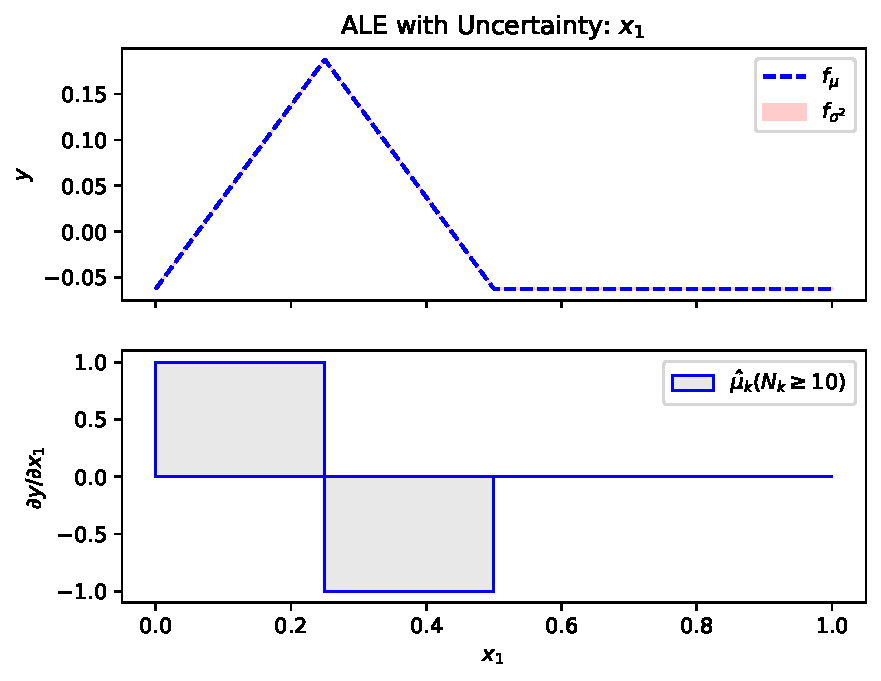
\includegraphics[width=.23\textwidth]{example_1/dale_feat_0.pdf}
  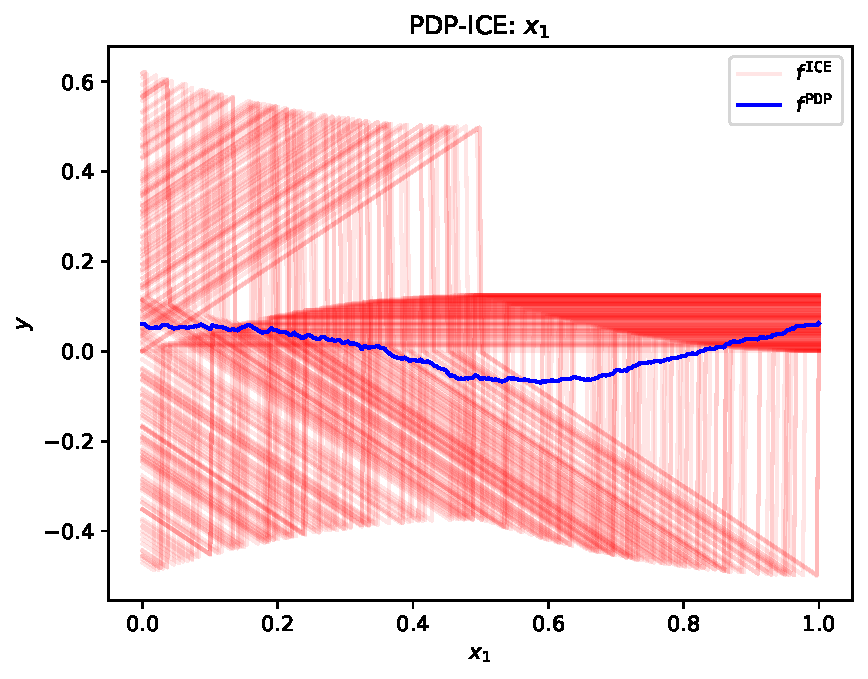
\includegraphics[width=.23\textwidth]{example_1/pdp_ice_feat_0.pdf}
  \caption{No interaction, Equal weights: Feature effect for \(x_1\);
    Ground-truth vs (a) UALE method at the left and (b) PDP-ICE at the
    right.}
  \label{fig:synth-ex-1-case-1}
\end{figure}

\paragraph{No Interaction, Different weights.}

As before, no interaction exits \(\alpha=0\), therefore, the
ground-truth uncertainty is zero, i.e.
\(f^{\mathcal{GT}}_{\sigma^2}(x_1) = 0\). The weigts are
\(a_1=2, a_2=0.5\), therefore, the ground-truth effect is
\(f_\mu^{\mathtt{GT}}(x_1)\) is, \(2x_1\) when \(0 \leq x_1 < 0.2\),
\(-2x_1\) when \(0.2 \leq x_1 < 0.4\) and zero otherwise. In
Figure~\ref{fig:ex-synth-1-2}, we observe that PDP estimation is
completely opposite to the ground-truth effect, i.e.~negative in the
region \([0, 0.2)\) and positive in \([0.2, 0.4)\), and the ICE
erroneously implies the existence of heterogeneous effects. As before,
ALE quantifies correctly the ground truth effect, the
zero-uncertainty and extracts the constant effect regions.

\begin{figure}[h]
  \centering
  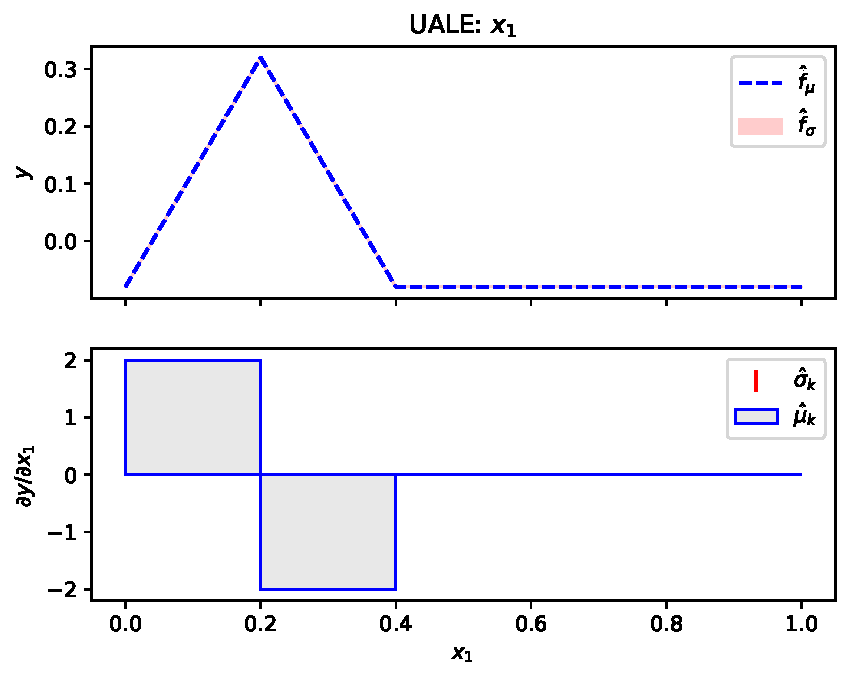
\includegraphics[width=.23\textwidth]{example_2/dale_feat_0.pdf}
  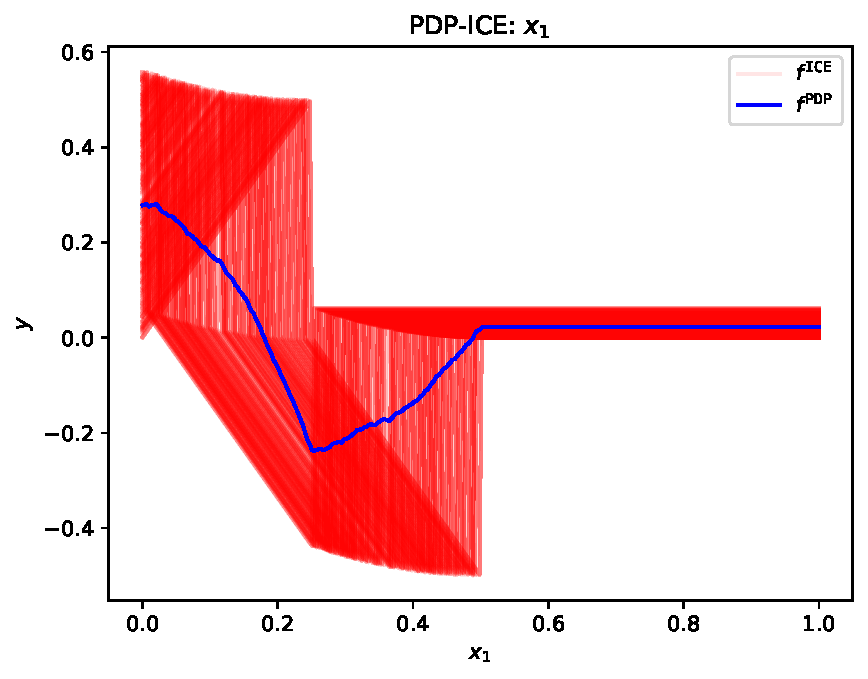
\includegraphics[width=.23\textwidth]{example_2/pdp_ice_feat_0.pdf}
  \caption{No interaction, Different weights: Feature effect for \(x_1\);
    Ground-truth vs (a) UALE method at the left and (b) PDP-ICE at the
    right.}
  \label{fig:ex-synth-1-2}
\end{figure}

\paragraph{Uncertainty, Equal weights.}

In this case we activate the interaction term, i.e. \(a=1\), and we
set the weights to \(a_1=a_2=1\). The interaction term provokes
heterogeneous effects for features \(x_1, x_3\), because the local
effects at \(x_1\) depend on the unknown value of \(X_3\) and
vice-versa. The effect of \(x_2\) has zero-uncertainty since it does
not appear in any interaction term. As we observe in
Figure~\ref{fig:ex-synth-1-3}, UALE correcly models the average effect
and the uncertainty in all cases. PDP-ICE quantifies correctly the
effect and the uncertainty only in the case of feature \(x_3\),
because \(X_3\) is independent from other features. For features
\(x_1, x_2\) that are correlated the average effect of PDP
and the uncertainty of ICE plots are wrong.

\begin{figure}[h]
  \centering
  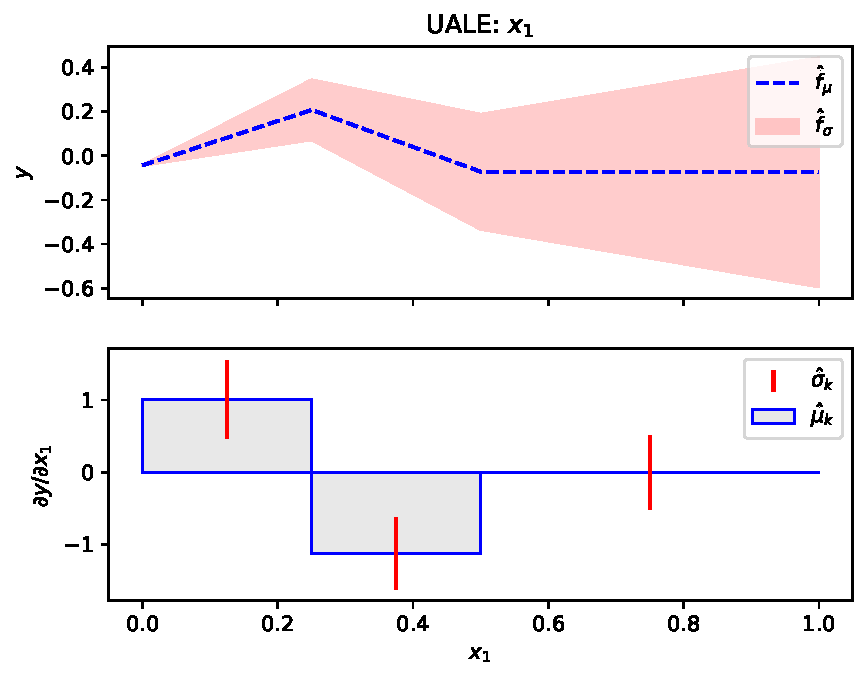
\includegraphics[width=.23\textwidth]{example_3/dale_feat_0.pdf}
  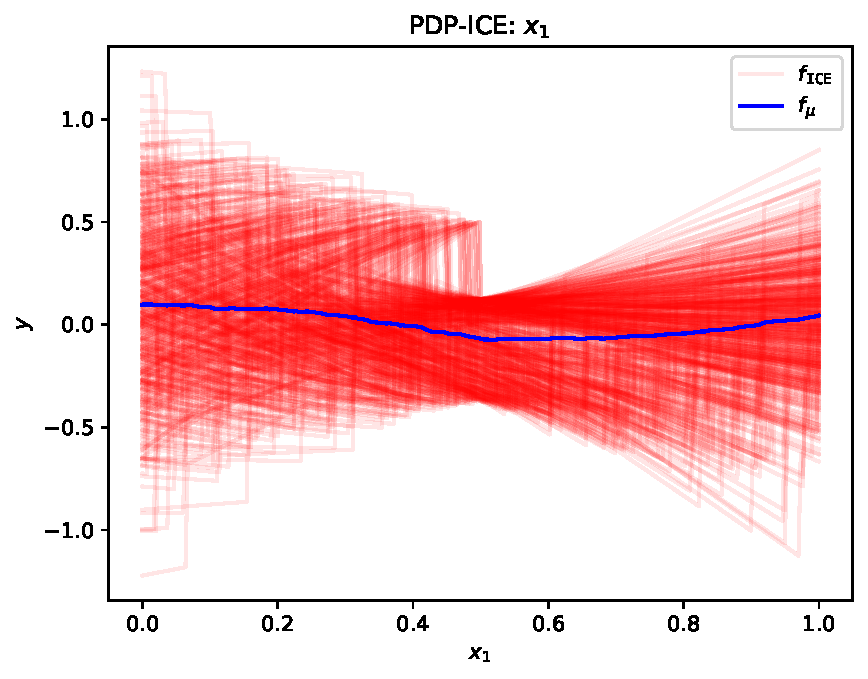
\includegraphics[width=.23\textwidth]{example_3/pdp_ice_feat_0.pdf}\\
  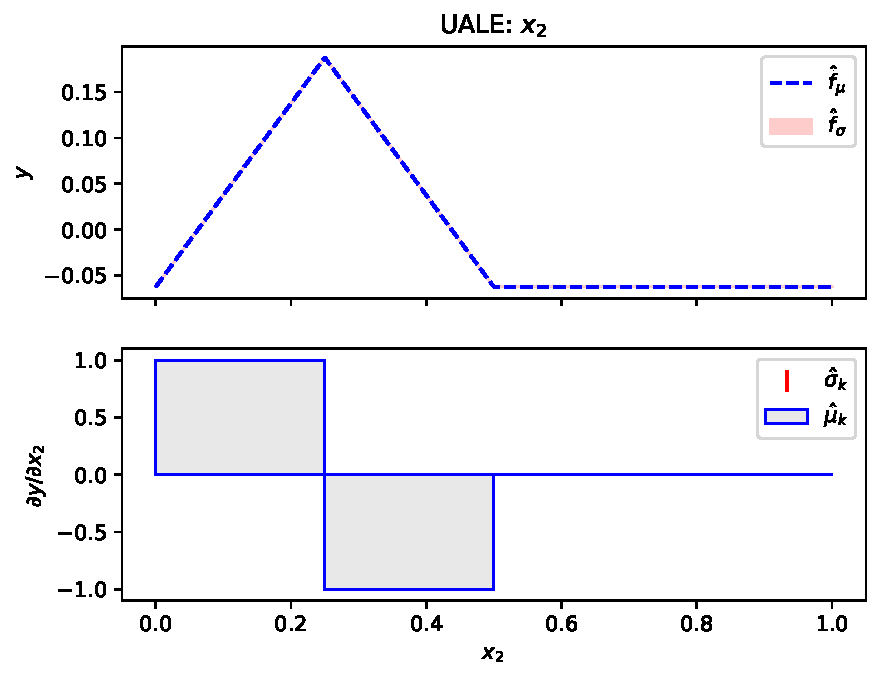
\includegraphics[width=.23\textwidth]{example_3/dale_feat_1.pdf}
  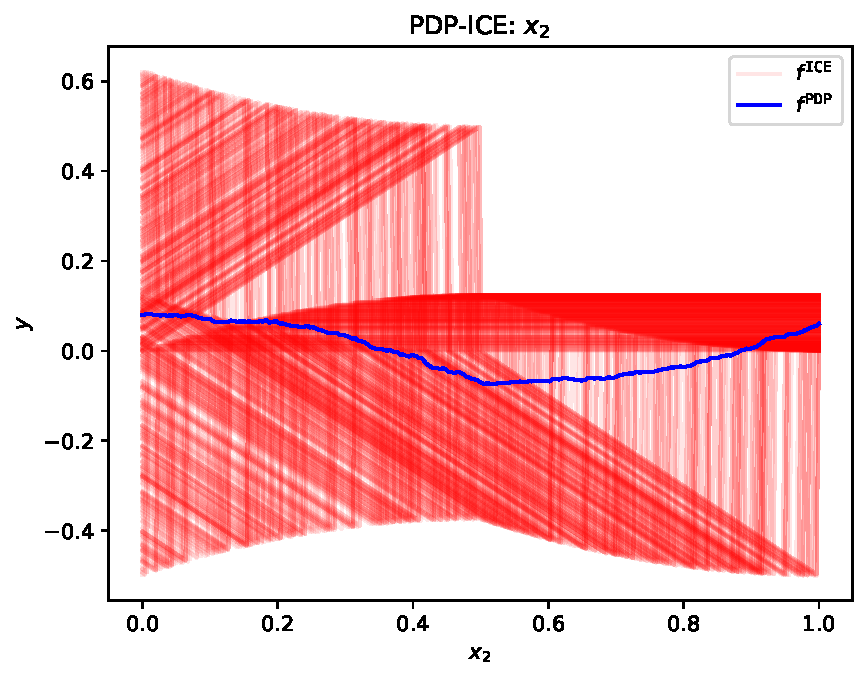
\includegraphics[width=.23\textwidth]{example_3/pdp_ice_feat_1.pdf}\\
  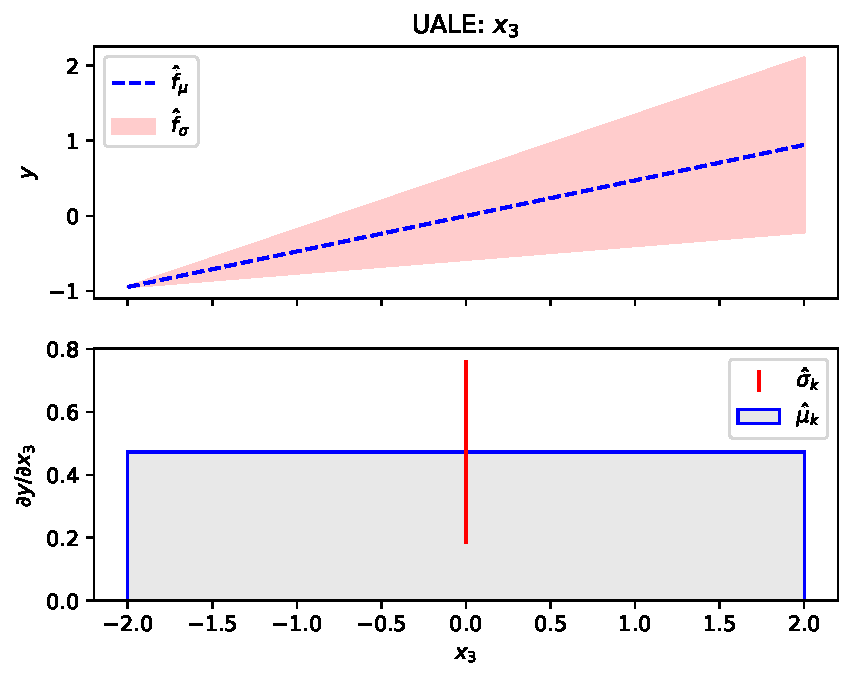
\includegraphics[width=.23\textwidth]{example_3/dale_feat_2.pdf}
  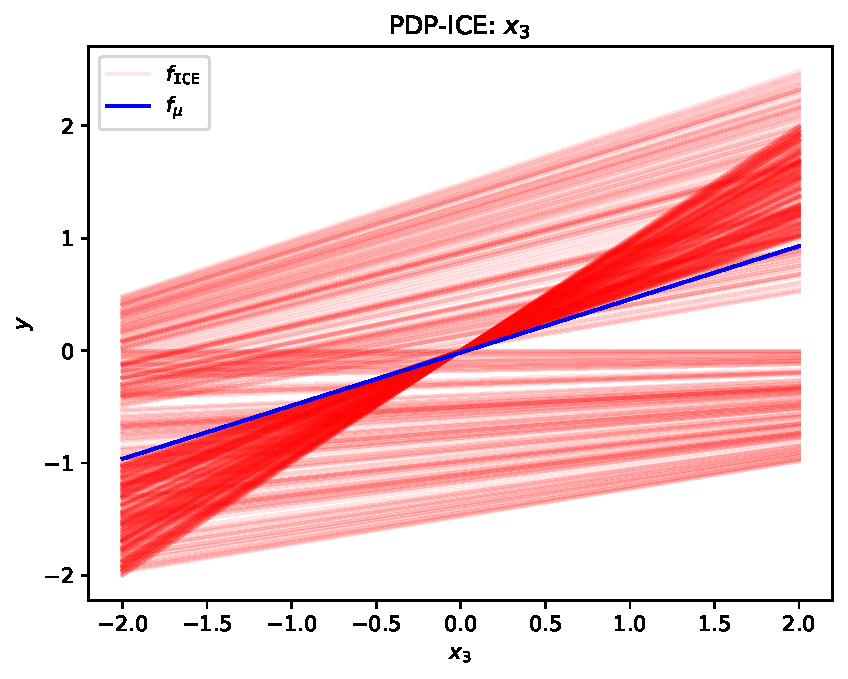
\includegraphics[width=.23\textwidth]{example_3/pdp_ice_feat_2.pdf}\\
  \caption{With interaction, equal weights: Feature effect for all
    features, \(x_1\) to \(x_3\) from top to bottom; Ground-truth vs
    (a) UALE method at the left columns and (b) PDP-ICE at the right
    column.}
  \label{fig:ex-synth-1-3}
\end{figure}

\paragraph{Discussion.}

Despite the model's simplicity, PDP-ICE fail in quantifying the
average effect and the uncertainty due to correlation between features
\(X_1\) and \(X_2\). UALE quantifies them correctly and estimates them
accurately extracting the regions with constant effect. The examples
above do not cover the case of an interaction term between correlated
features, e.g. \(x_1x_2\), because there is an open debate about the
ground-truth effect in this case~\citep{Gromping2020MAEP}.

\subsection{Case 2: Bin-Splitting}
\label{sec:simulation-examples-2}

In this simulation, we aim to to quantify the advantages of automatic
bin-splitting. We set-up the following validation framework. We
generate a big dataset with dense sampling (\(N=10^6\)) and we treat
the DALE estimation with dense fixed-size bins (\(K=10^3\)) as
ground-truth. Afterwards, we generate less samples (\(N=500\)) and we
compare the fixed-size DALE estimation (for many different \(K\))
versus the automatic bin-splitting. In all cases, we use a bivariate
black-box function \(f(\cdot)\) where the samples are instances of the
distribution \(p(\mathbf{x}) = p(x_2|x_1)p(x_1)\) where
\(x_1 \sim \mathcal{U}(0,1)\) and
\(x_2 \sim \mathcal{N}(x_1, \sigma_2^2=0.5)\). We denote as
\(\mathcal{Z^{\mathtt{DP}}} = \{z^{\mathtt{DP}}_{k-1}, \cdots,
z^{\mathtt{DP}}_{K}\}\) the sequence obtained by automatic
bin-splitting and with \(\mathcal{Z^{\mathtt{K}}}\) the fixed-size
splitting with \(K\) bins.  For consistent results, in all the
examples below, we regenerate samples and repeat the computations for
\(t = 30\) times, providing the mean value for all metrics.

\paragraph{Metrics}

The evaluation is done with regard to two metrics that count the mean
bin error, where bin error is the absolute difference of the
approximation from the ground-truth. The metric
\(\mathcal{L}_{\mathtt{DP|K}}^{\mu} =
\frac{1}{|\mathcal{Z}^{\mathtt{DP|K}}|} \sum_{k \in
  \mathcal{Z}^{\mathtt{DP|K}}} | \mu_k - \hat{\mu}_k | \) counts the
mean bin error on the average effect and
\(\mathcal{L}_{\mathtt{DP|K}}^{\sigma} =
\frac{1}{|\mathcal{Z}^{\mathtt{DP|K}}|} \sum_{k \in
  \mathcal{Z}^{\mathtt{DP|K}}} | \sigma_k - \hat{\sigma}_k | \) the
mean bin error on the uncertainty. In both cases the ground truth is
computed from the dense bins of ground-truth that overlapse with the
wider bin of the approximation. We also provide the mean (per bin)
error term
\(\mathcal{L}^{\rho}_{\mathtt{DP|K}} =
\frac{1}{|\mathcal{Z}^{\mathtt{DP|K}}|} \sum_{k \in
  \mathcal{Z}^{\mathtt{DP|K}}} \rho_k \) for a complete understanding
of the uncertainty error. 

\paragraph{Piecewise-Linear Function.}

In this example, we define \(f(\mathbf{x}) = a_1x_1 + x_1x_2\) with
\(5\) piecewise-linear regions of different-size, i.e., \(a_1\) equals
to \(=\{2, -2, 5, -10, 0.5\}\) in the intervals defined by the
sequence \(\{0, 0.2, 0.4, 0.45, 0.5, 1\}\). As we observe, in
Figure~\ref{fig:ex-synth-2-1}, UALE method extracts a sequence of
intervals with better \(\mathcal{L}_{\mathtt{DP}}^{\mu}\) and
\(\mathcal{L}_{\mathtt{DP}}^{\sigma^2}\) error compared to any
fixed-size splitting. Analyzing the fixed-size errors helps us
understand the importance of variable-size splitting. In
Figure~\ref{fig:ex-synth-2-1}(b), we observe a positive trend between
\(\mathcal{L}^{\mu}_{\mathtt{K}}\) and \(K\), concluding that bin
effect estimation is more incosistent as \(\Delta x\) becomes smaller,
due to less points contributing to each bin. The interpretation of
variance error is slightly more complex. Given that the smallest
interval is \(\Delta x = 0.05 \Rightarrow K = 20\) and all intervals
are multiples of the smallest interval, any \(K\) that is not a
multiple of \(20\) adds nuisance uncertainty
\(\mathcal{L}^{\rho^2}_{\mathtt{K}}\) leading to a high variance error
\(\mathcal{L}^{\sigma^2}_{\mathtt{K}}\). In these cases, the variance
error reduces as \(K\) grows bigger because the length of the bins
that lie in the limit between two piecewise linear regions becomes
smaller. For \(K=\{20, 40, 60, 80, 100\}\) where
\(\mathcal{L}^{\rho^2}_{\mathtt{K}} \approx 0\), we conclude the same
as with with the mean effect error, i.e. the estimation becomes more
incosistent as \(K\) grows larger.

Variable-size extracts correctly the fine-grain bins, e.g., intervals
\([0.4, 0.45]\), \([0.45, 0.5]\), and acts as a merging mechanism to
create wider bins when the effect remains constant, e.g. interval
\([0.5, 1]\), leading to an optimal solution.

\begin{figure}[h]
  \centering
  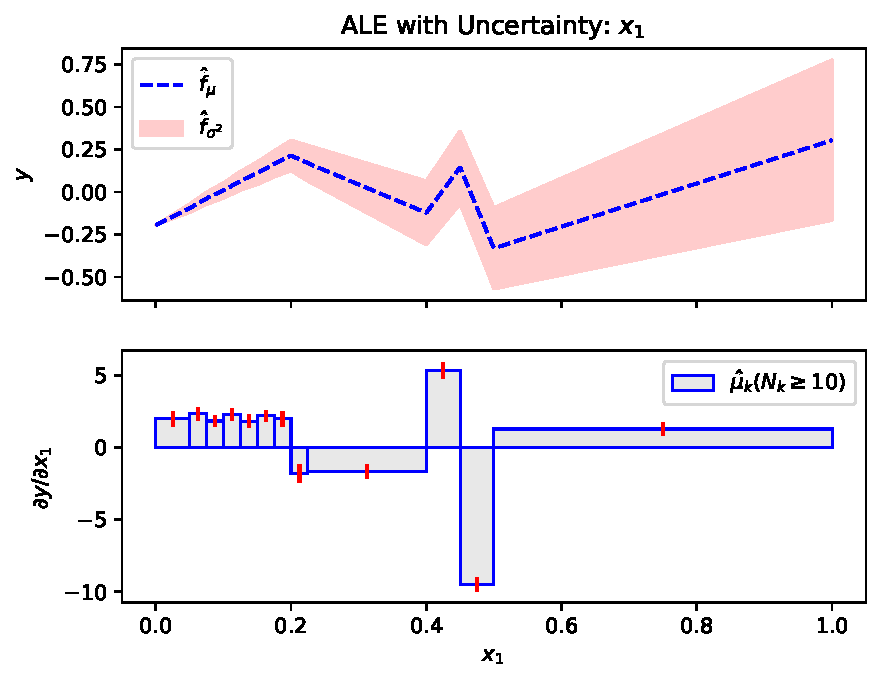
\includegraphics[width=.23\textwidth]{example_bin_splitting_1/fig_1.pdf}
  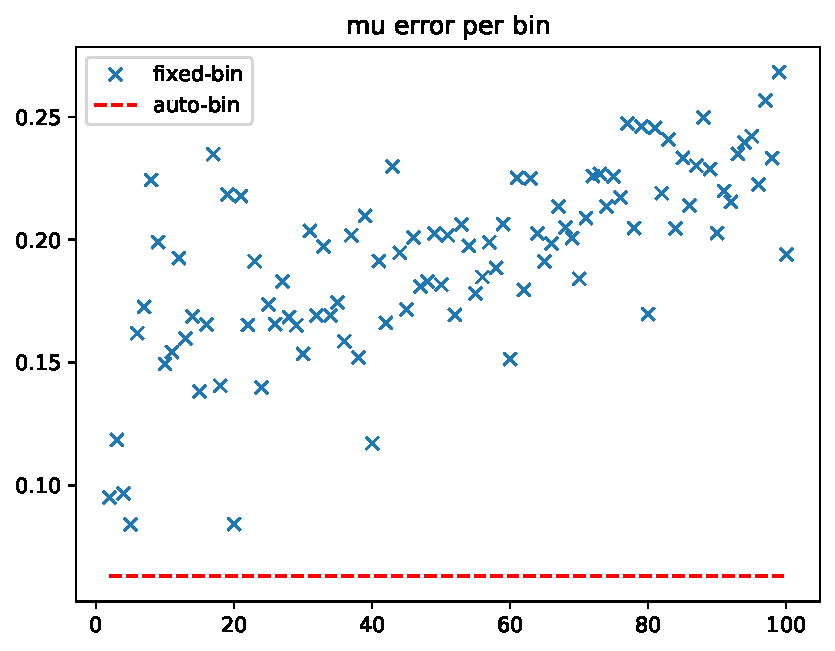
\includegraphics[width=.23\textwidth]{example_bin_splitting_1/fig_2.pdf}\\
  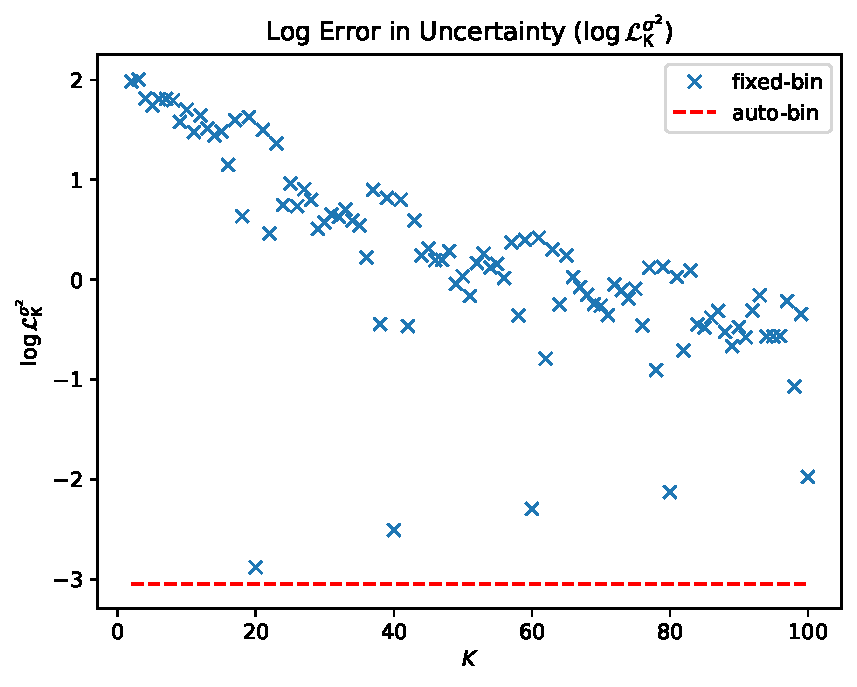
\includegraphics[width=.23\textwidth]{example_bin_splitting_1/fig_3.pdf}
  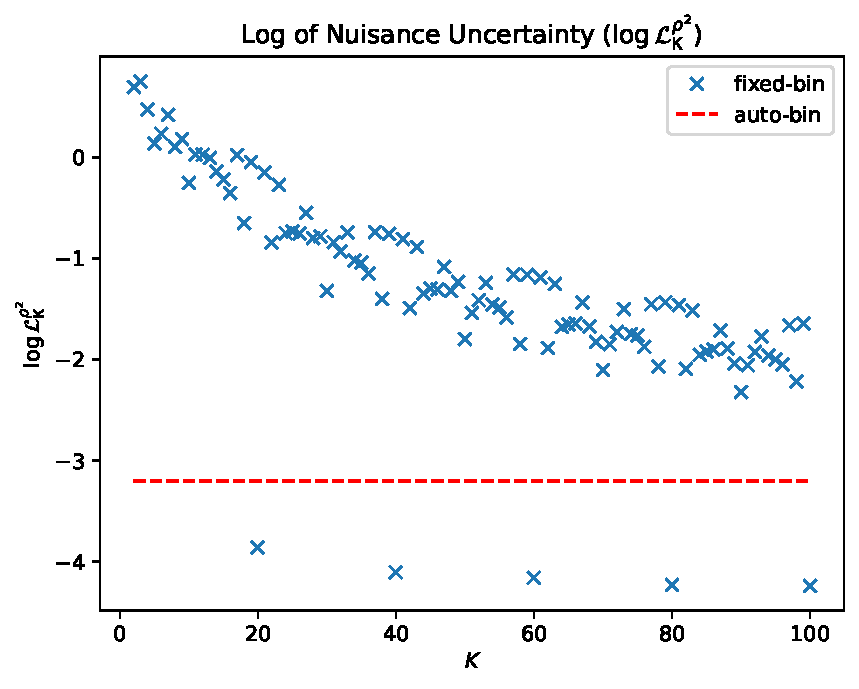
\includegraphics[width=.23\textwidth]{example_bin_splitting_1/fig_4.pdf}
  \caption{Figure 1}
  \label{fig:ex-synth-2-1}
\end{figure}


\paragraph{Non-Linear Function.}

In this example, we define a black-box function
\(f(\mathbf{x}) = 4x_1^2 + x_2^2 + x_1x_2\), where the effect is
non-linear in all the range of \(x\). This case has two
specialties. First, there is no obvious advantage of variable-size
versus fixed-size splitting, and, second, there is not an apriori
optimal bin-size. Widening a bin will increase the resolution error
\(\mathcal{L}^{\rho^2}\) and narrowing will make less robust. In
Figure~\ref{fig:ex-synth-2-2}, we observe that automatic bin splitting
finds a solution that compromises the conflicting objectives, i.e., it
keeps as low as possible both the main effect
\(\mathcal{L}^{\mu}_{\mathtt{K}}\) and the variance error
\(\mathcal{L}^{\sigma^2}_{\mathtt{K}}\).

\begin{figure}[h]
  \centering
  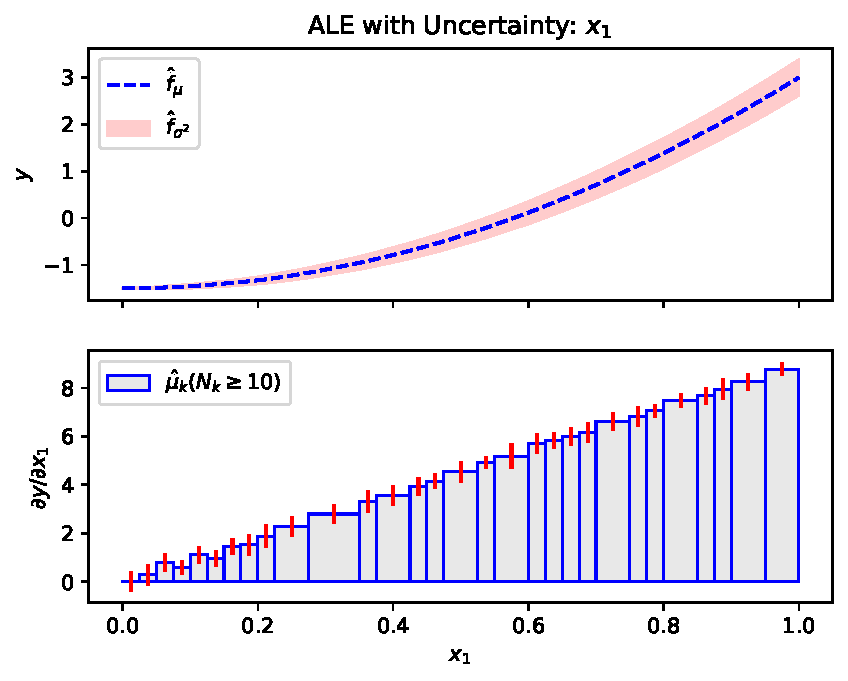
\includegraphics[width=.23\textwidth]{example_bin_splitting_2/fig_1.pdf}
  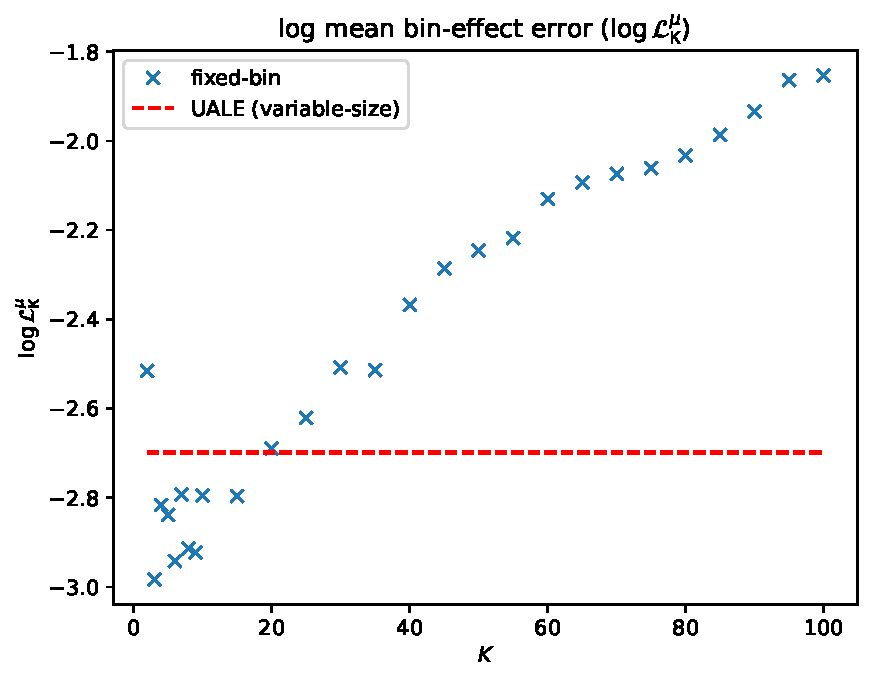
\includegraphics[width=.23\textwidth]{example_bin_splitting_2/fig_2.pdf}\\
  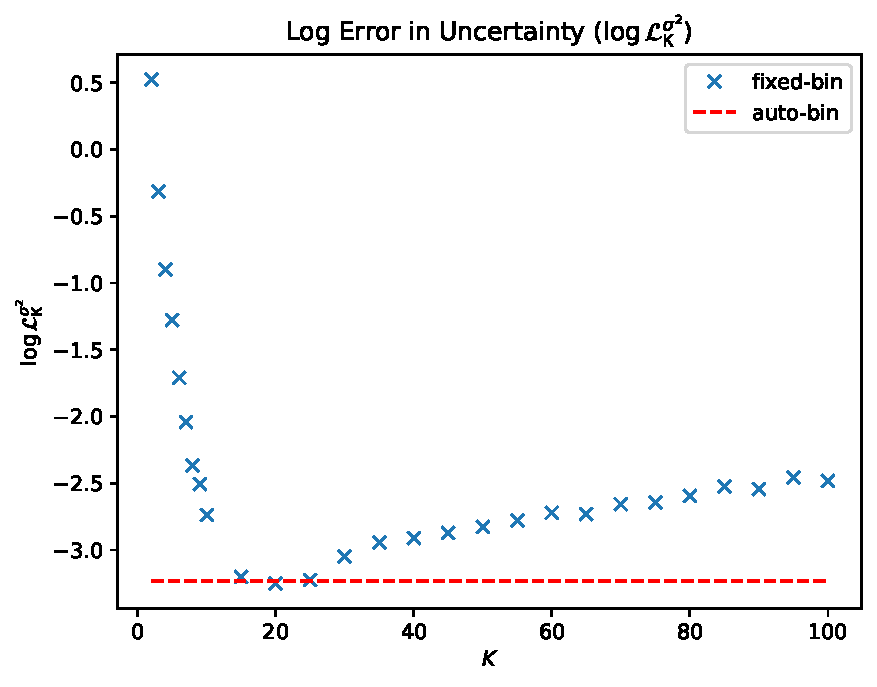
\includegraphics[width=.23\textwidth]{example_bin_splitting_2/fig_3.pdf}
  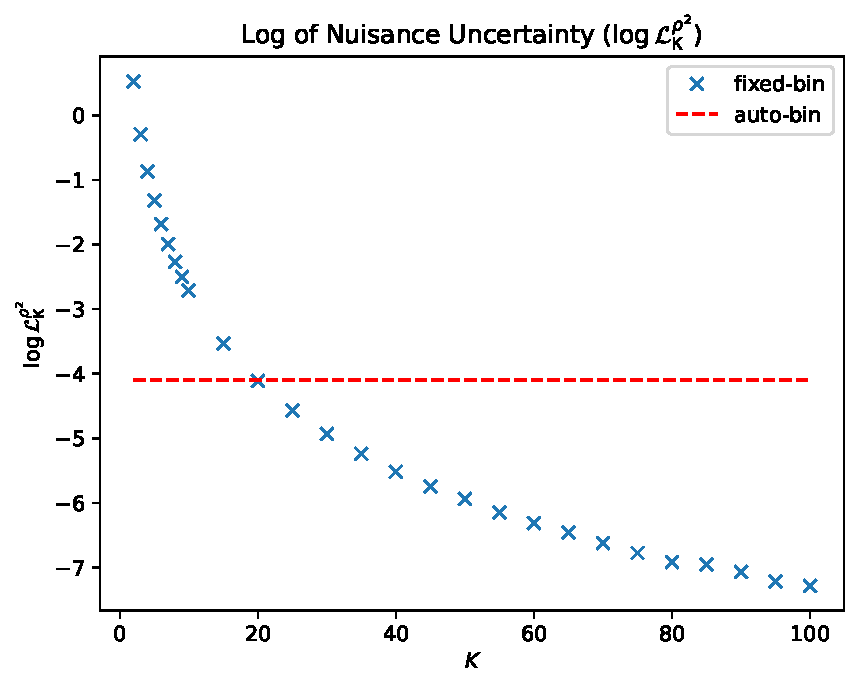
\includegraphics[width=.23\textwidth]{example_bin_splitting_2/fig_4.pdf}
  \caption{Figure 1}
  \label{fig:ex-synth-2-2}
\end{figure}

\section{REAL-WORLD EXAMPLE}

Here, we aim at demonstrating the usefuleness of uncertainty
quantification and the advantages of automatic bin-splitting, on the
real-world California Housing dataset~\citep{pace1997sparse}.

\paragraph{ML setup}

The California Housing is a largely-studied dataset with approximately
\(20000\) training instances, making it appropriate for robust
Monte-Carlo approximations. The dataset contains \(D=8\) numerical
features with characteristics about the building blocks of California,
e.g. latitude, longitude, population of the block or median age of
houses in the block. The target variable is the median value of the
houses inside the block in dollars that ranges between
\([15, 500] \cdots 10^3\), with a mean value of
\(\mu_Y \approx 201 \cdot 10^3 \) and a standard deviation of
\(\sigma_Y \approx 110 \cdot 10^3\).


We exclude instances with missing values or with outlier values. As
outlier we define the feature values which ar over three standard
deviations away from the mean feature value. We also normalize all
features to zero-mean and unit standard deviation. We split the
dataset into \(N_{tr} = 15639\) training and \(N_{test} = 3910\) test
examples (80/20 split) and we fit a Neural Network with 3 hidden
layers of 256, 128 and 36 units respectively. After 15 epochs using
the Adam optimizer with learning rate \(\eta = 0.02\), the model
achieves a normalized mean squared error (R-Squared) of \(0.25\)
(0.75), which corresponds to a MAE of \(37 \cdot 10^3\) dollars. 

Below, we illustrate the feature effect for three features: latitude
\(x_2\), population \(x_6\) and median income \(x_8\). The particular
features cover the main FE cases, e.g.~positive/negative trend and
linear/non-linear curve, and they are appropriate for illustration
purposes. The complete results for all features, along with in-depth
information about the preprocessing, training and evaluation parts are
provided in the Appendix.

\paragraph{Uncertainty Quantification}

In real-world datasets, it is infeasible to obtain the ground truth FE
for seamlessly evaluating the competitive methods. We selected the
particular experiment, because, in broad terms, UALE and PDP-ICE plots
aggree in the estimation of the average effect and
uncertainty. Therefore, we can focus on juding the quality of the
information provided by the two methods.

In Figure\ref{fig:ex-real-1}, we observe, from top to bottom, the
effects for the latitude, population and the median income. The effect
of UALE and PDP-ICE are similar for the population and the median
income. The population has a negative impact that progressively
decreases: from 400 to 1500 people the house value decreases with a
rate of \(-150 (\pm 140)\) dollars per added person, a rate that
decreases from \(-80 (\pm 80)\) to \(-60 (\pm 60)\) dollars per added
person as we move from 1500 to 2800 people. The level of uncertainty
indicates significant variance in absolute value of the rate, but in
the grant majority of instances the rate is negative. With the same
inspection, we observe that the median annual income has a positive
impact on the value (all numbers are thousands of dollars):
\(20\pm 15\) per \(10\) of added median income for incomes in
\([8, 15]\), \(32 \pm 20\) per \(10\) added income in \([15, 60]\) and
\(40 \pm 15\) per \(10\) added income in \([60, 70]\). The uncertainty
indicates that there are less heterogeneous effects about the median
income compared to the number of people. In both cases, we can end-up
to the same conclusion by inspecting the PDP-ICE plots. For the
latitude, there is a small difference in the explanations for the
region \([32, 35]\), where UALE estimates a less negative slope with
less uncertainty than PDP, while the explanations are similar for the
range \([35,39]\), where both methods reveal an increase in the
uncertainty around the feature value \(37.5\).

In general, we observe that UALE complements ALE in the quantification
of the heterogeneous effects, similarly to as ICE complements PDP. The
automatic extraction of constant-effect and constant-uncertainty
regions provided by UALE is helpful for an easier interpretation. On
the other hand, ICE plots sometimes are more descritive on locating
the type of heterogeneity, whereas UALE quantifies only the level (not
the type) of heterogeneity.

\begin{figure}[h]
  \centering
  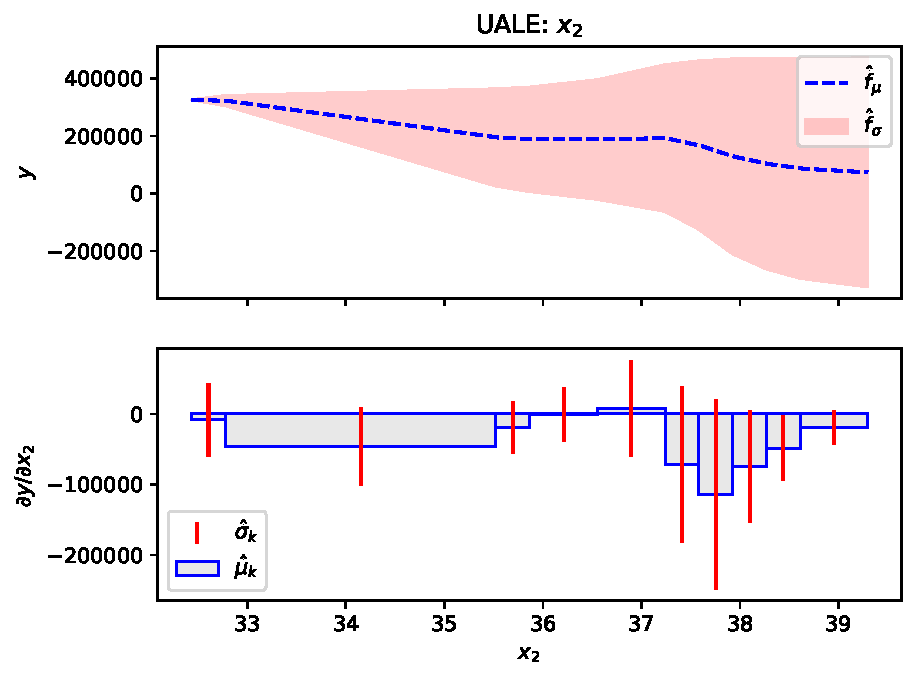
\includegraphics[width=.23\textwidth]{real_dataset_3/feature_1_ale_auto.pdf}
  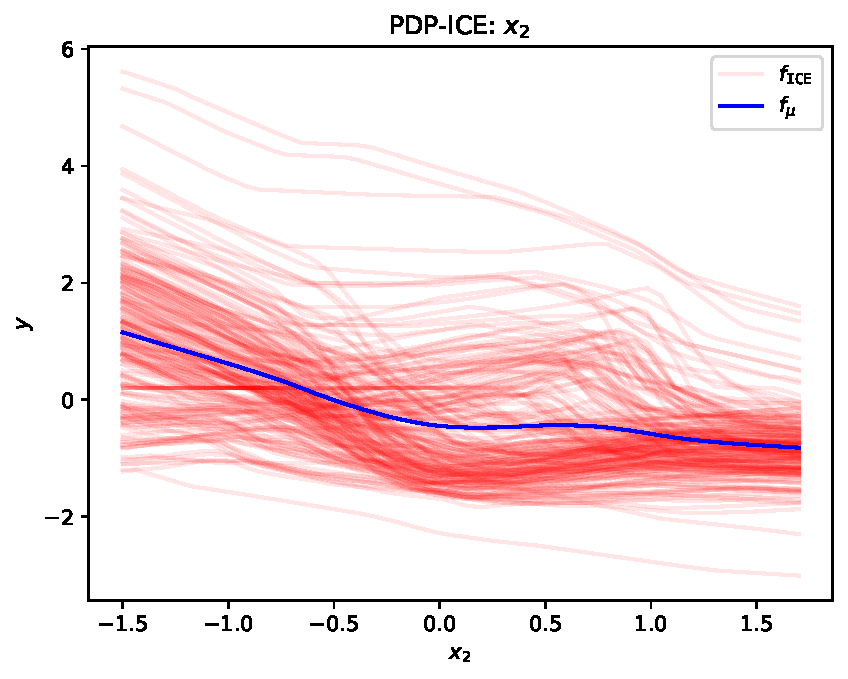
\includegraphics[width=.23\textwidth]{real_dataset_3/feature_1_pdp_ice.pdf}\\
  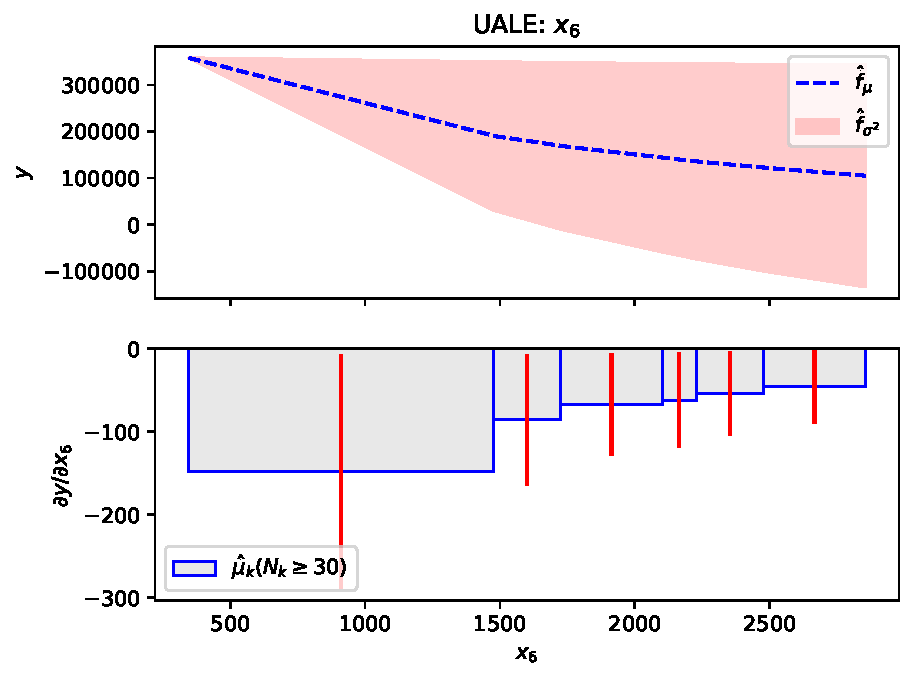
\includegraphics[width=.23\textwidth]{real_dataset_3/feature_5_ale_auto.pdf}
  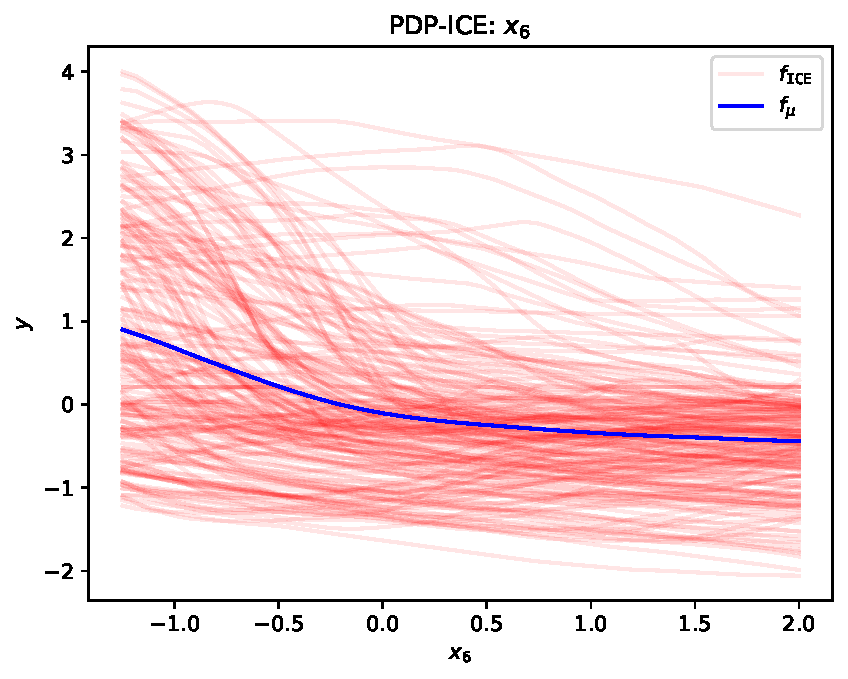
\includegraphics[width=.23\textwidth]{real_dataset_3/feature_5_pdp_ice.pdf}\\
  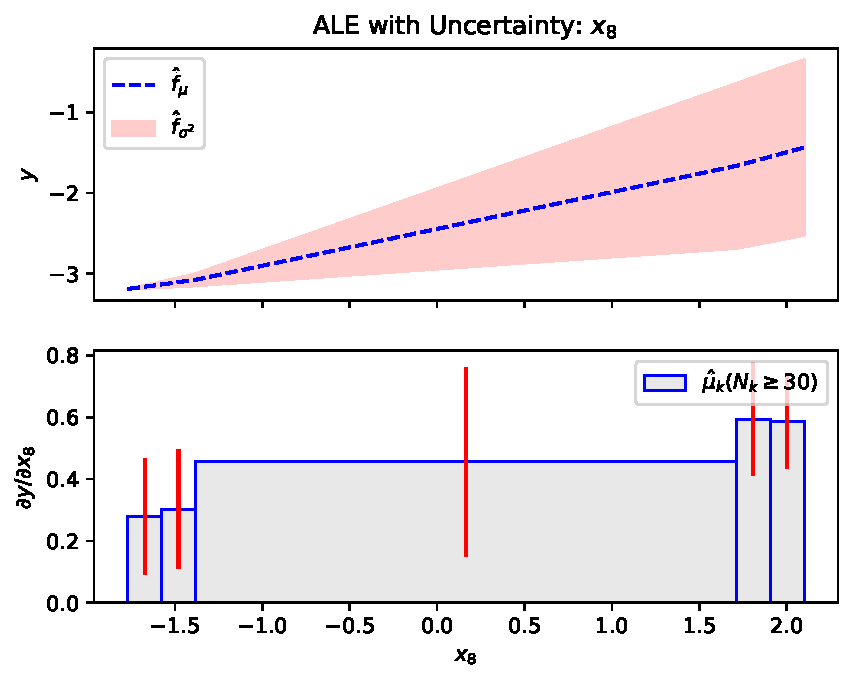
\includegraphics[width=.23\textwidth]{real_dataset_3/feature_7_ale_auto.pdf}
  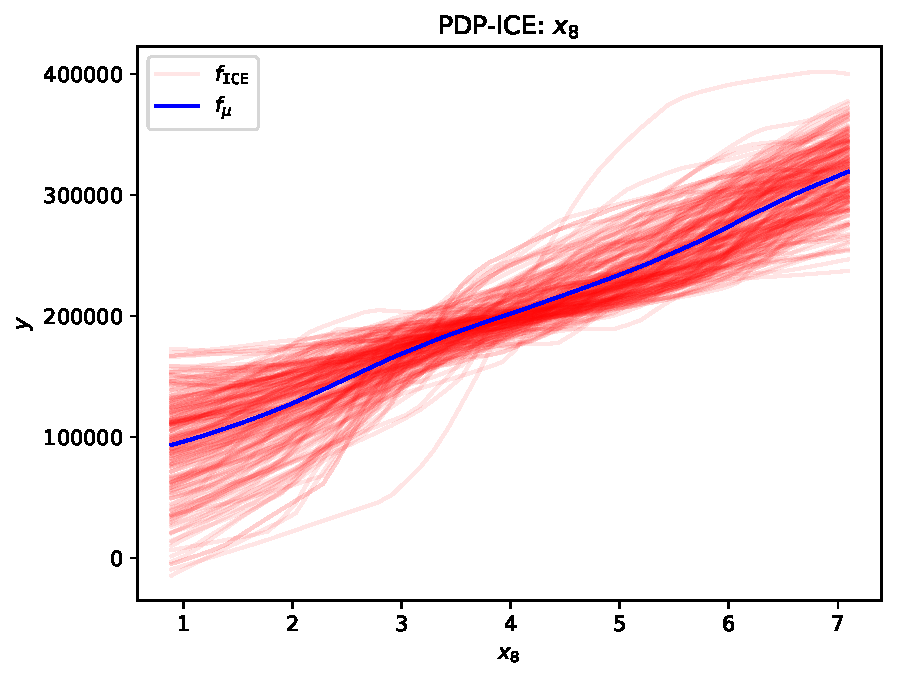
\includegraphics[width=.23\textwidth]{real_dataset_3/feature_7_pdp_ice.pdf}\\
  \caption{Figure 1}
  \label{fig:ex-real-1}
\end{figure}

\paragraph{Bin Splitting}

In this part, we evaluate the robustness of the approximation using
automatic bin-splitting. Following the evaluation framework of
Section~\ref{sec:simulation-examples-2}, we treat as ground-truth the
effects computed on the full training-set \(N=20000\) with dense
fixed-size bin-splitting (\(K=80\)). Given the big number of samples,
we make the hypothesis that the approximation with dense binning is
close to the ground truth. Afterwards, we randomly select less samples
\(N=1000\) and we compare UALE approximation with all possible
fixed-size alternatives, repeating this process for 30 times for
robust results. In Figure~\ref{fig:ex-real-2}, we illustrate the mean
values for \(\mathcal{L}^{\mu}, \mathcal{L}^{\sigma}\) of the 30
repetitions. We observe that automatic bin-spliting provides (close to
the) best approximation in the three features. In the Appendix, we
provide the same evaluation for all features.

\begin{figure}[h]
  \centering
  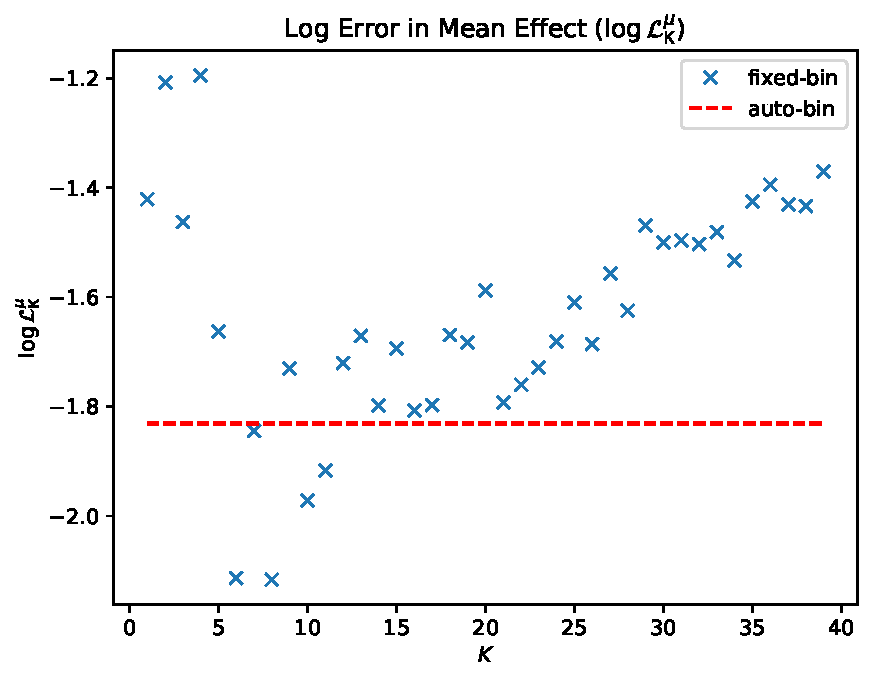
\includegraphics[width=.23\textwidth]{real_dataset_3/compare_mu_err_feature_1.pdf}
  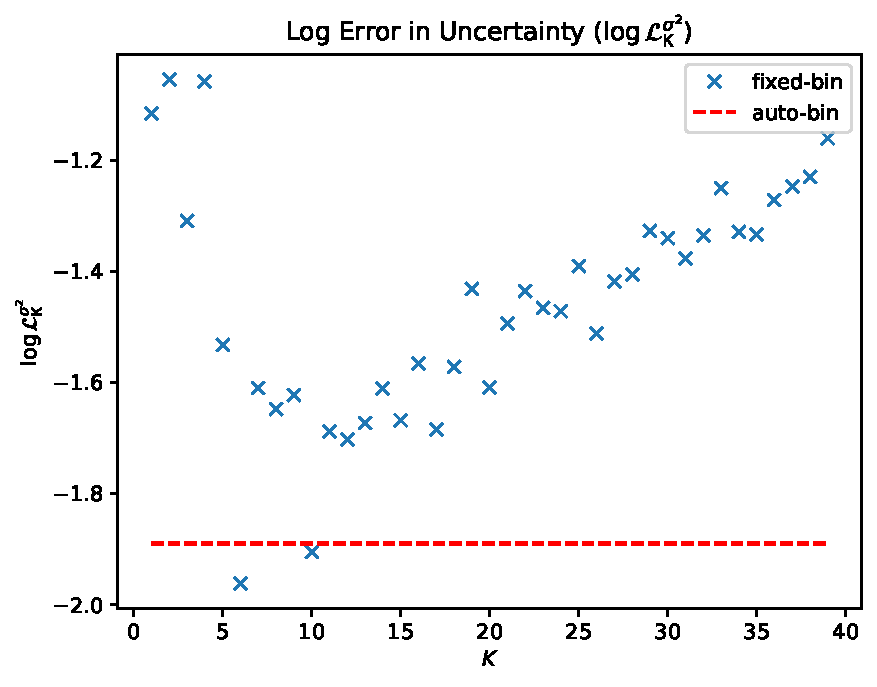
\includegraphics[width=.23\textwidth]{real_dataset_3/compare_var_err_feature_1.pdf}\\
  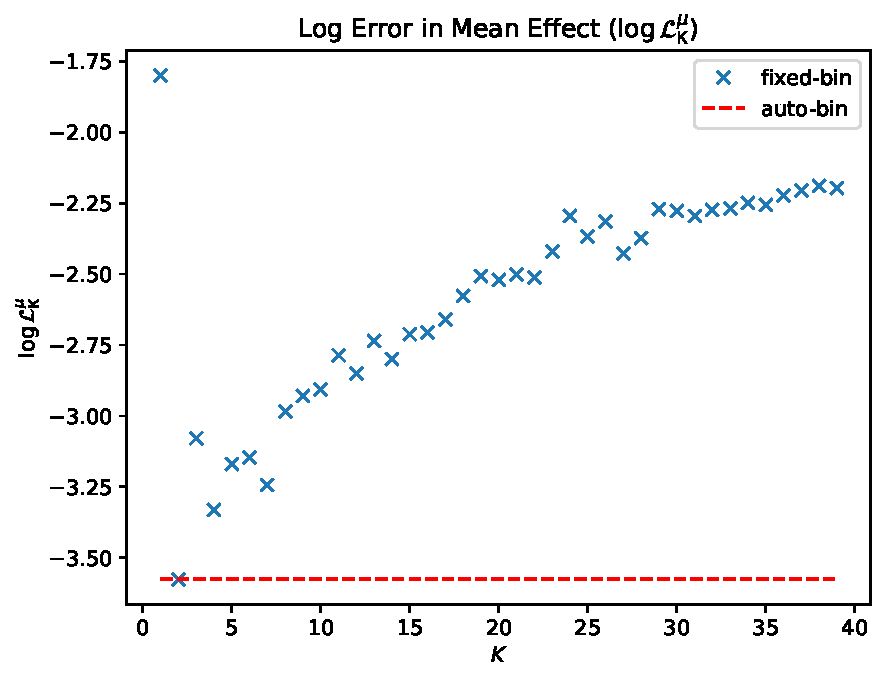
\includegraphics[width=.23\textwidth]{real_dataset_3/compare_mu_err_feature_5.pdf}
  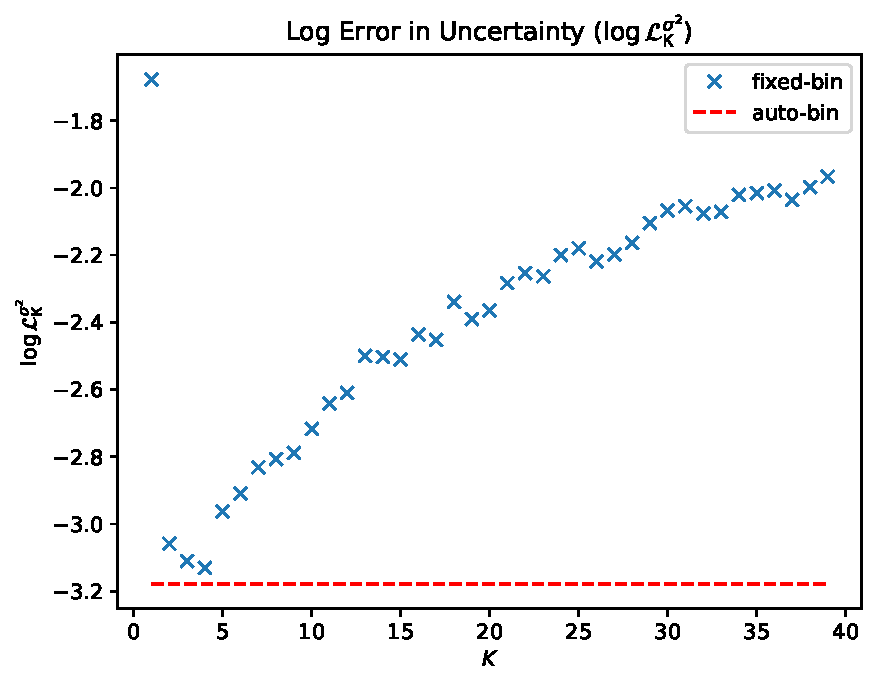
\includegraphics[width=.23\textwidth]{real_dataset_3/compare_var_err_feature_5.pdf}\\
  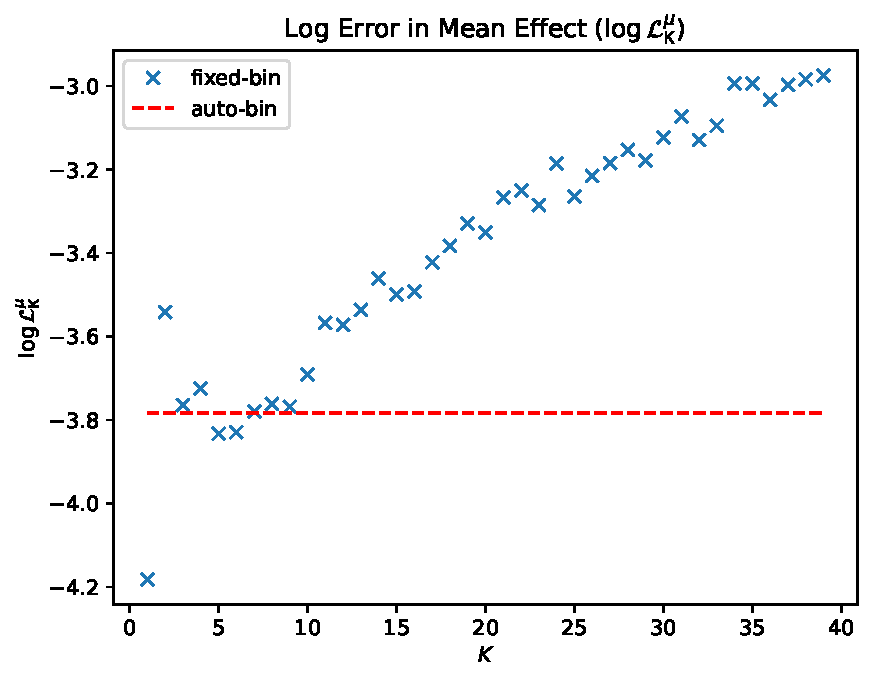
\includegraphics[width=.23\textwidth]{real_dataset_3/compare_mu_err_feature_7.pdf}
  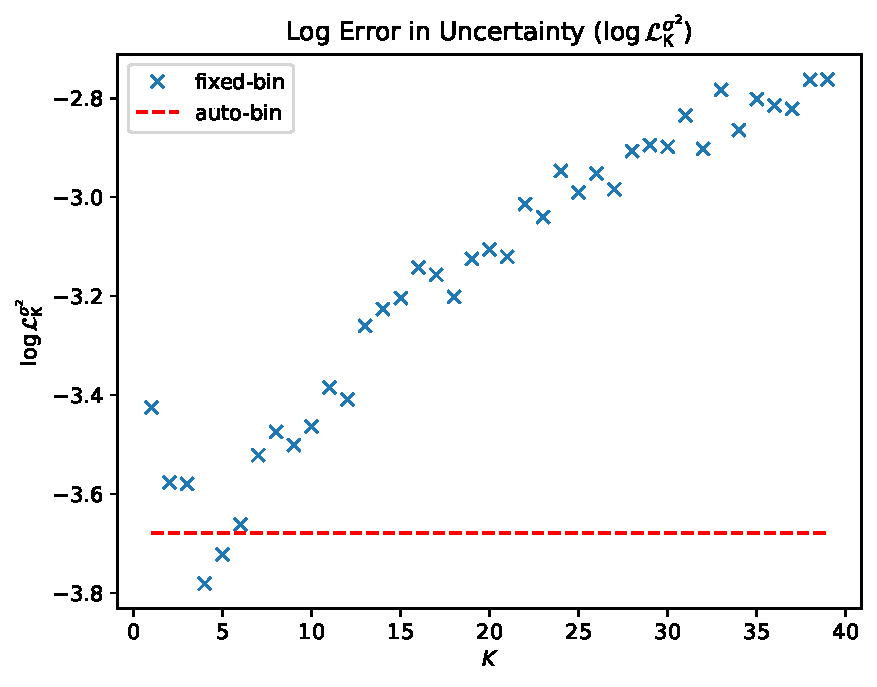
\includegraphics[width=.23\textwidth]{real_dataset_3/compare_var_err_feature_7.pdf}\\
  \caption{Figure 1}
  \label{fig:ex-real-2}
\end{figure}

\section{DISCUSSION}

add limitations.

\subsubsection*{Acknowledgments}
All acknowledgments go at the end of the paper, including thanks to reviewers who gave useful comments, to colleagues who contributed to the ideas, and to funding agencies and corporate sponsors that provided financial support. 
To preserve the anonymity, please include acknowledgments \emph{only} in the camera-ready papers.

\bibliography{biblio}

\end{document}
